\section*{Preguntas}
\begin{multicols}{2}
\begin{enumerate}
	
	\item La fuerza normal es aquella que actúa en dirección \rule{3cm}{0.5pt} a una superficie.
	\begin{enumerate}[a)]
		\item Paralela
		\item \colorbox[rgb]{1,1,0}{Perpendicular}
		\item Antiparalela
		\item NAC
	\end{enumerate}
	
	
	
	\item La primera Ley de Newton enuncia que la velocidad de un cuerpo en equilibrio es:
	\begin{enumerate}[a)]
		\item Variante
		\item Constante
		\item Cero
		\item \colorbox[rgb]{1,1,0}{B y C}
		\item NAC
	\end{enumerate}
	
	
	
	\item Suponga que habla con un teléfono interplanetario a un amigo que vive en la Luna. Él le dice que acaba de ganar un newton de oro en un concurso. Con emoción, ¡Usted le dice que entró a la versión terricola del mismo concurso y qe también ganó un newton de oro! ¿quién es más rico?
	\begin{enumerate}[a)]
		\item Usted
		\item \colorbox[rgb]{1,1,0}{Su amigo}
		\item Ambos son igualmente ricos
		\item NAC
	\end{enumerate}
	
	\columnbreak
	
	\item Una utiliza una báscula para medir su peso en un elevador, ¿cuándo le da la lectura máxima? Cuando el elevador: 
	\begin{enumerate}[a)]
		\item Sube con $v$ constante
		\item \colorbox[rgb]{1,1,0}{Acelera hacia arriba}
		\item Acelera hacia abajo
		\item Baja con $v$ constante
		\item NAC
	\end{enumerate}
	
	
	
	\item Un bloque de masa ”m” descansa sobre un plano inclindao con un ángulo  ¿Cuál de los siguientes enunciados es correcto?
	\begin{enumerate}[a)]
		\item La fuerza normal es igual al peso
		\item \colorbox[rgb]{1,1,0}{La fuerza normal es menor al peso}
		\item La fuerza normal es mayor al peso
		\item No se puede saber, faltan datos
		\item NAC
	\end{enumerate}
	
	
	
\end{enumerate}
\end{multicols}



\pagebreak

\section*{Problema}
Una gran bola para demolición está sujeta por dos cables de acero ligeros. Si su masa $m$ es de $4090 kg$, calcule la tensión del cable horizontal ($T_A$).

\begin{figure}[H]
	\centering
	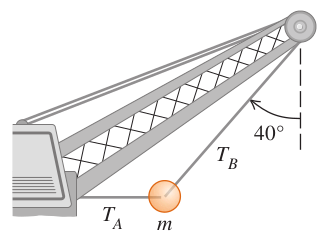
\includegraphics[scale=0.5]{./img/bola.png}
\end{figure}

\vspace{1cm}

\textbf{Respuesta: } \colorbox[rgb]{1,1,0}{$3.36\times 10^{4} N$}























%%%%